\documentclass[a4paper,10pt,notitlepage]{article}
\usepackage{ctex,geometry,graphicx,tikz,setspace,paralist,fancyhdr,caption}
\geometry{
	left=1.5cm,
	right=1.5cm,
	top=1.4cm,
	bottom=2cm,}
\newcommand{\rec}{
	\begin{tikzpicture}[remember picture,overlay]
		% 绘制边框
		\draw[line width=1.2pt] ([xshift=0.5cm,yshift=0.5cm] current page.south west) rectangle ([xshift=-0.5cm,yshift=-0.8cm] current page.north east);
	\end{tikzpicture}
	
}
\pagestyle{fancy}
\fancyhf{}
\fancyhead[C]{\rec}  % 在页眉中绘制图形
\fancyhead[L]{模电实验报告}
\fancyhead[R]{实验六 \quad 比例求和运算电路}
\fancyfoot[C]{\thepage}
\begin{document}
	\large
	\onehalfspacing
	\begin{figure}[h]
		\raggedright
		
\includegraphics{1.png}
	\end{figure}
	\centering
	{\Huge\textbf{模电实验报告}\par}
	\vspace{0.2cm}
	{\huge{实验内容:比例求和运算电路}\par}
	\raggedright
	\vspace{0.3cm}
	\begin{centering}
		{\large 院系:电子与信息工程学院\hfill 学号:22309080\hfill 审批:\hspace{2cm} \par
			专业:通信工程\hfill 实验人:梁倍铭\hfill 日期:2023年11月18日 \par}
	\end{centering}
	\vspace{0.3cm}
	\section*{一、实验目的}
	\begin{enumerate}
		\item 了解运算放大器的基本使用方法。
		\item 应用集成运放构成基本运算电路,并测定它们输出信号与输入信号间运算关系。
		\item 学会使用线性组件741。
	\end{enumerate}
	\section*{二、原理简介}
	\begin{enumerate}
		\item 反相比例放大器\par 
		\qquad 电路如图6-1 所示,当运算放大器开环放大倍数足够大时(大于104 以上),反相比例
		放大器的闭环电压放大倍数为:$$A_{uf}=\frac{u_o}{u_i}=-\frac{R_F}{R_1}$$
		\begin{figure}[h]
			\centering
			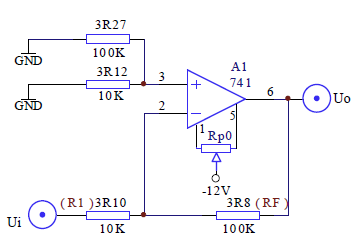
\includegraphics[width=0.5\textwidth]{2.png}
			\caption*{图6-1 }
		\end{figure}
		\qquad 由上式可知,选用不同的电阻比值,Auf 可以大于1,也可以小于1,若取RF=R1,则
		放大器的输出电压等于输入电压的负值,也称为反相跟随器。
		\item 同相比例放大器\par 
		\qquad 电路如图6-2 所示,当运算放大器开环放大倍数足够大时(大于104 以上),同相比例
		放大器的闭环电压放大倍数为:$$A_{uf}=\frac{u_o}{u_i}=\frac{R_F}{R_1}$$
		\qquad 由上式可知,选用不同的电阻比值,Auf 可以大于1,也可以小于1,若取RF=R1,则
		放大器的输出电压等于输入电压,也称为跟随器。
		\begin{figure}[h]
			\centering
			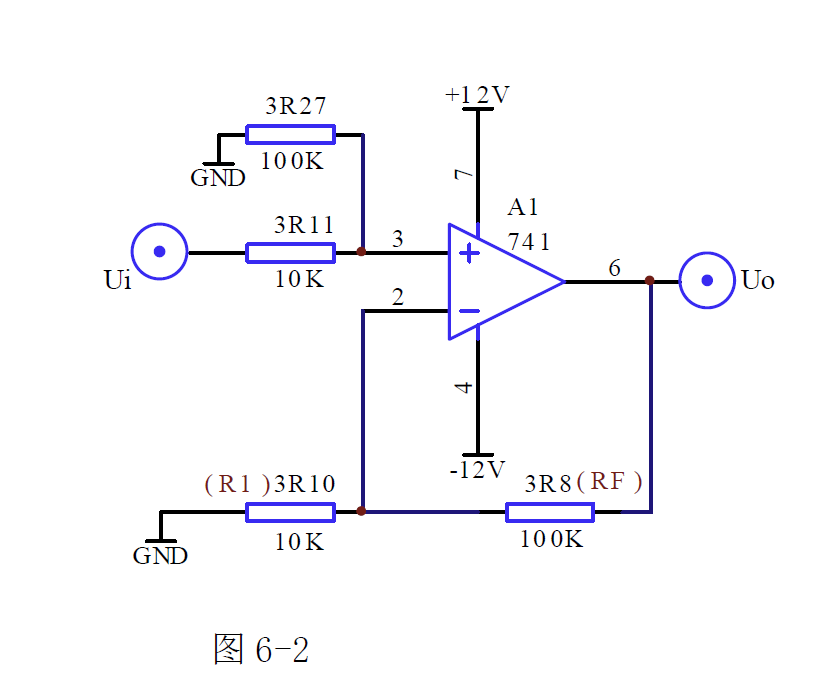
\includegraphics[width=0.5\textwidth]{3.png}
			\caption*{图6-2 }
		\end{figure}
		\item 减法器(差分比例运算)\par 
		\qquad 电路如图6-3 所示,当运算放大器开环增益足够大时(大于104 以上),,输出电压Uo
		为: $$u_o=-\frac{R_F}{R_1}(u_{i1}-u_{i2})$$
		\begin{figure}[h]
			\centering
			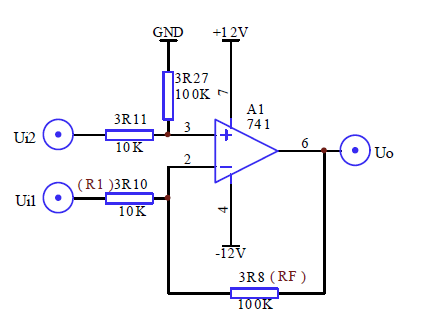
\includegraphics[width=0.5\textwidth]{4.png}
			\caption*{图6-3 }
		\end{figure}
		\item  反相加法器\par 
		\qquad 电路如图6-4 所示,当运算放大器开环增益足够大时(大于104 以上),,输出电压Uo
		为: $$u_o=-\frac{R_F}{R_1}(u_{i1}-u_{i2})$$
		\begin{figure}[h]
			\centering
			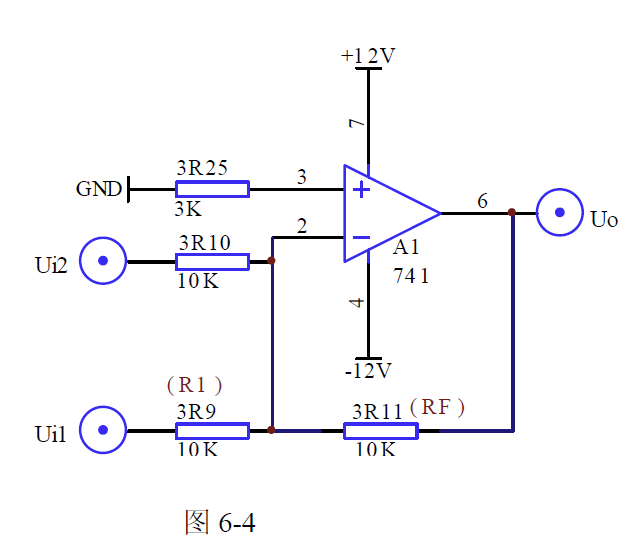
\includegraphics[width=0.5\textwidth]{5.png}
			\caption*{图6-4 }
		\end{figure}
		\item 加减法器\par 
		\qquad 电路如图6-5 所示,当运算放大器开环增益足够大时(大于104 以上),,输出电压Uo
		为: $$u_o=R_{F2}(\frac{u_{i1}}{R_1}+\frac{u_{i2}}{R_2}-\frac{u_{i3}}{R_3})$$
		\begin{figure}[h]
			\centering
			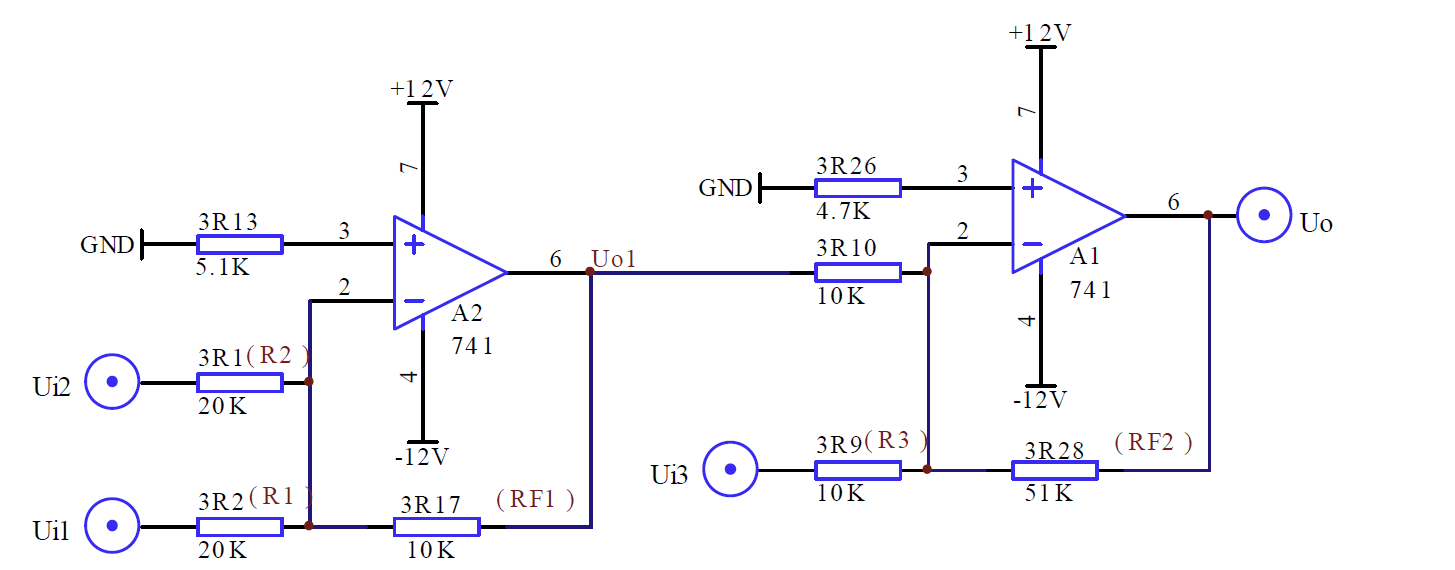
\includegraphics[width=0.8\textwidth]{6.png}
			\caption*{图6-5 }
		\end{figure}
	\end{enumerate}
	\section*{三、实验器材}
	1、 实验箱 2、数字万用表 3、函数信号发生器 4、交流毫伏表5、双踪示波器
	\section*{四、实验步骤和内容}
	\begin{enumerate}
		\item 调零\par 
		按图6-1 连接电路,直流电源供电为±12V。将Ui 对地短路,接通电源后,调节调零
		电位器Rp0(10K),使输出Uo=0,然后将短路线去掉。
		\item  反相比例放大器 \par 
		\begin{enumerate}
			\item 在步骤1 的基础上,按给定直流输入信号,测量对应的输出电压,把结果记入表
			6-1 中。
			\begin{table}[h]
				\centering
				\begin{tabular}{|c|c|c|c|c|c|c|c|}
					\hline
					\multicolumn{2}{|c|}{$U_i(V)$} & 0.3 & 0.5 & 0.7 & 1.0 & 1.1 & 1.2 \\
					\hline
					理论计算值 & $U_O(V)$ & -2.99 & -4.99 & -7.00 & -10 & -10.9 & -11.6 \\
					\hline
					实际测量值 & $U_O(V)$ & -3.0025 & -5.065 & -6.946 & -9.912 & -10.056 & -10.10 \\
					\hline
					实际放大倍数 & $A_{uf}$ & -10.008 & -10.13 & -9.923 & -9.912 & -9.14 & -8.425 \\
					\hline
				\end{tabular}
				\caption*{表6-1 反相比例放大器}
			\end{table}
			\item 在该比例放大器的输入端加入1KHz, 有效值为0.5V 的交流信号,用示波器观察
			输出波形,并与输入波形相比较。
			\begin{figure}[h]
				\raggedright
				\begin{minipage}{0.3\textwidth}
					\centering
					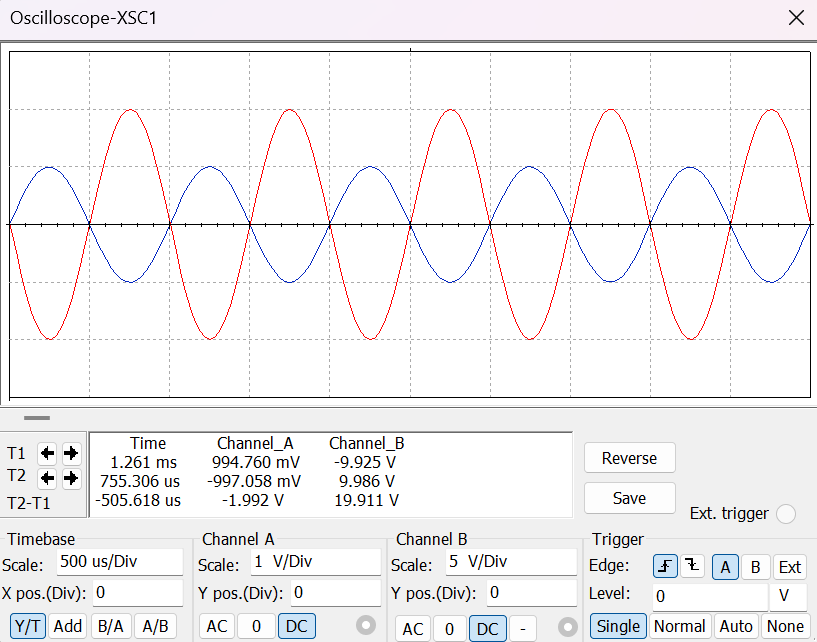
\includegraphics[width=\textwidth]{预习报告/3.png}
					\caption*{图6-6 输入输出仿真波形}
				\end{minipage}
				\qquad
				\begin{minipage}{0.3\textwidth}
					\centering
					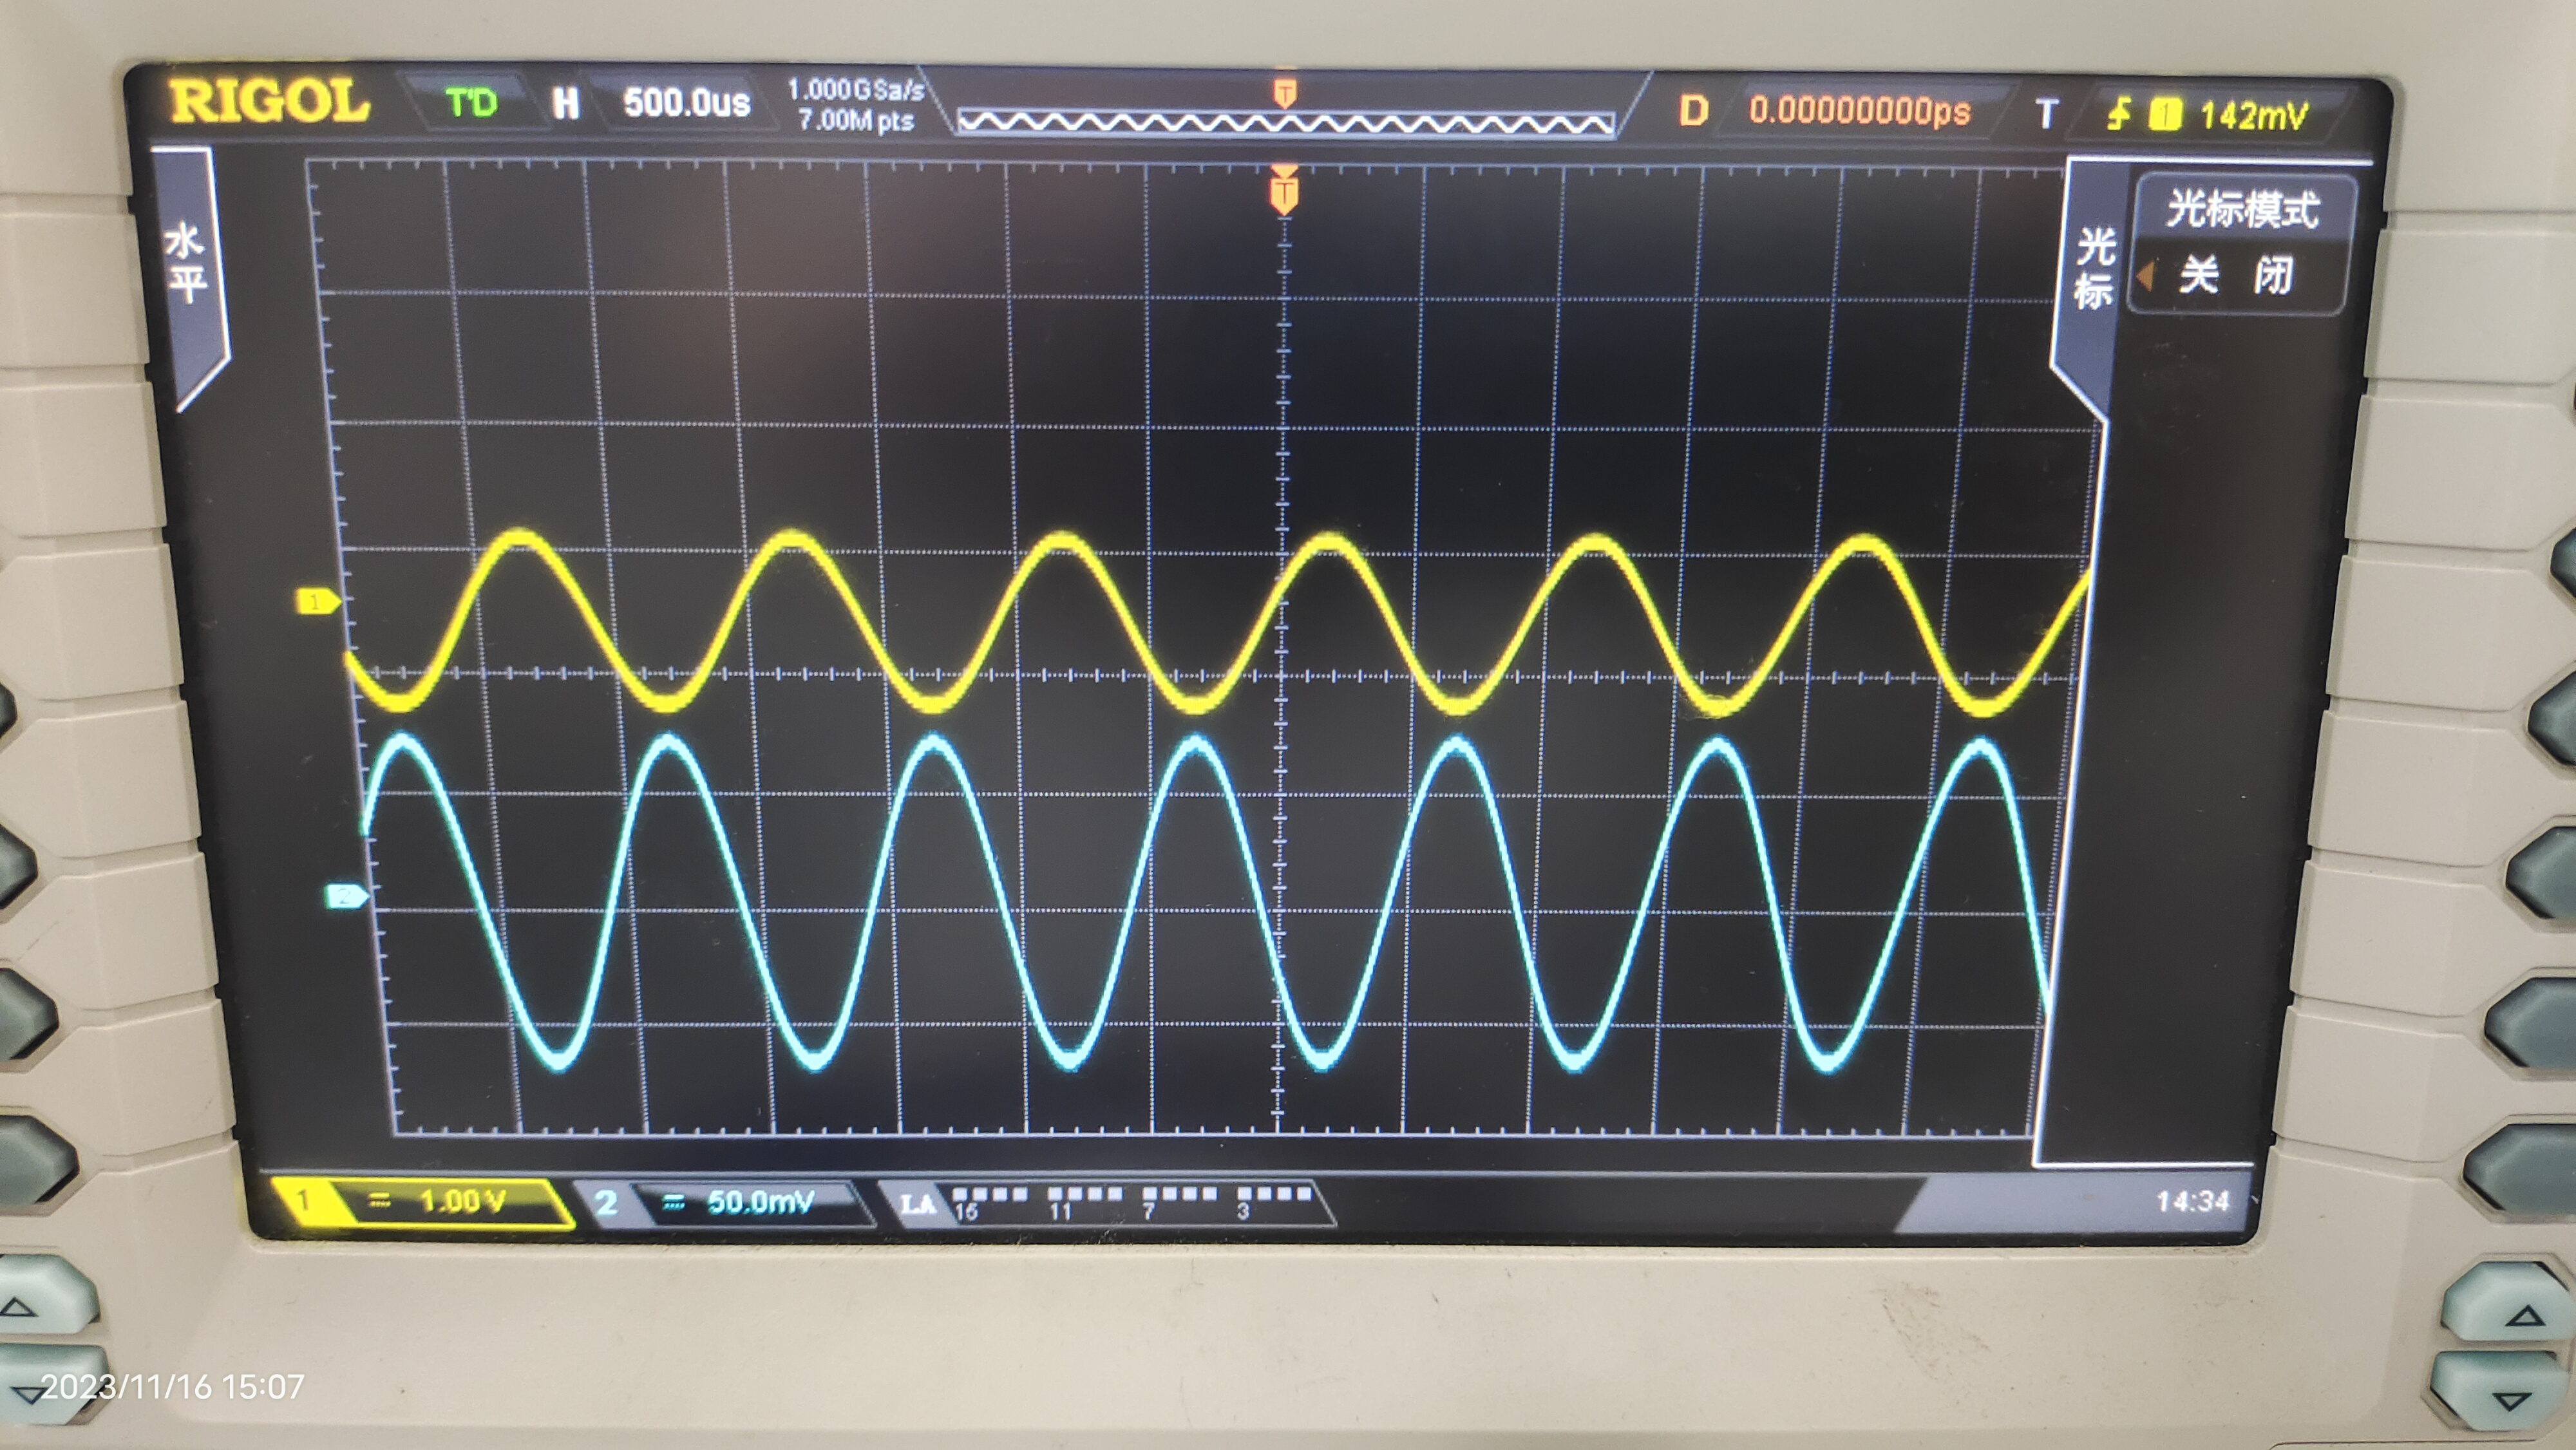
\includegraphics[width=\textwidth]{1.jpg}
					\caption*{图6-7 输入输出实验波形}
				\end{minipage}
				\qquad
				\begin{minipage}{0.3\textwidth}
					\centering
					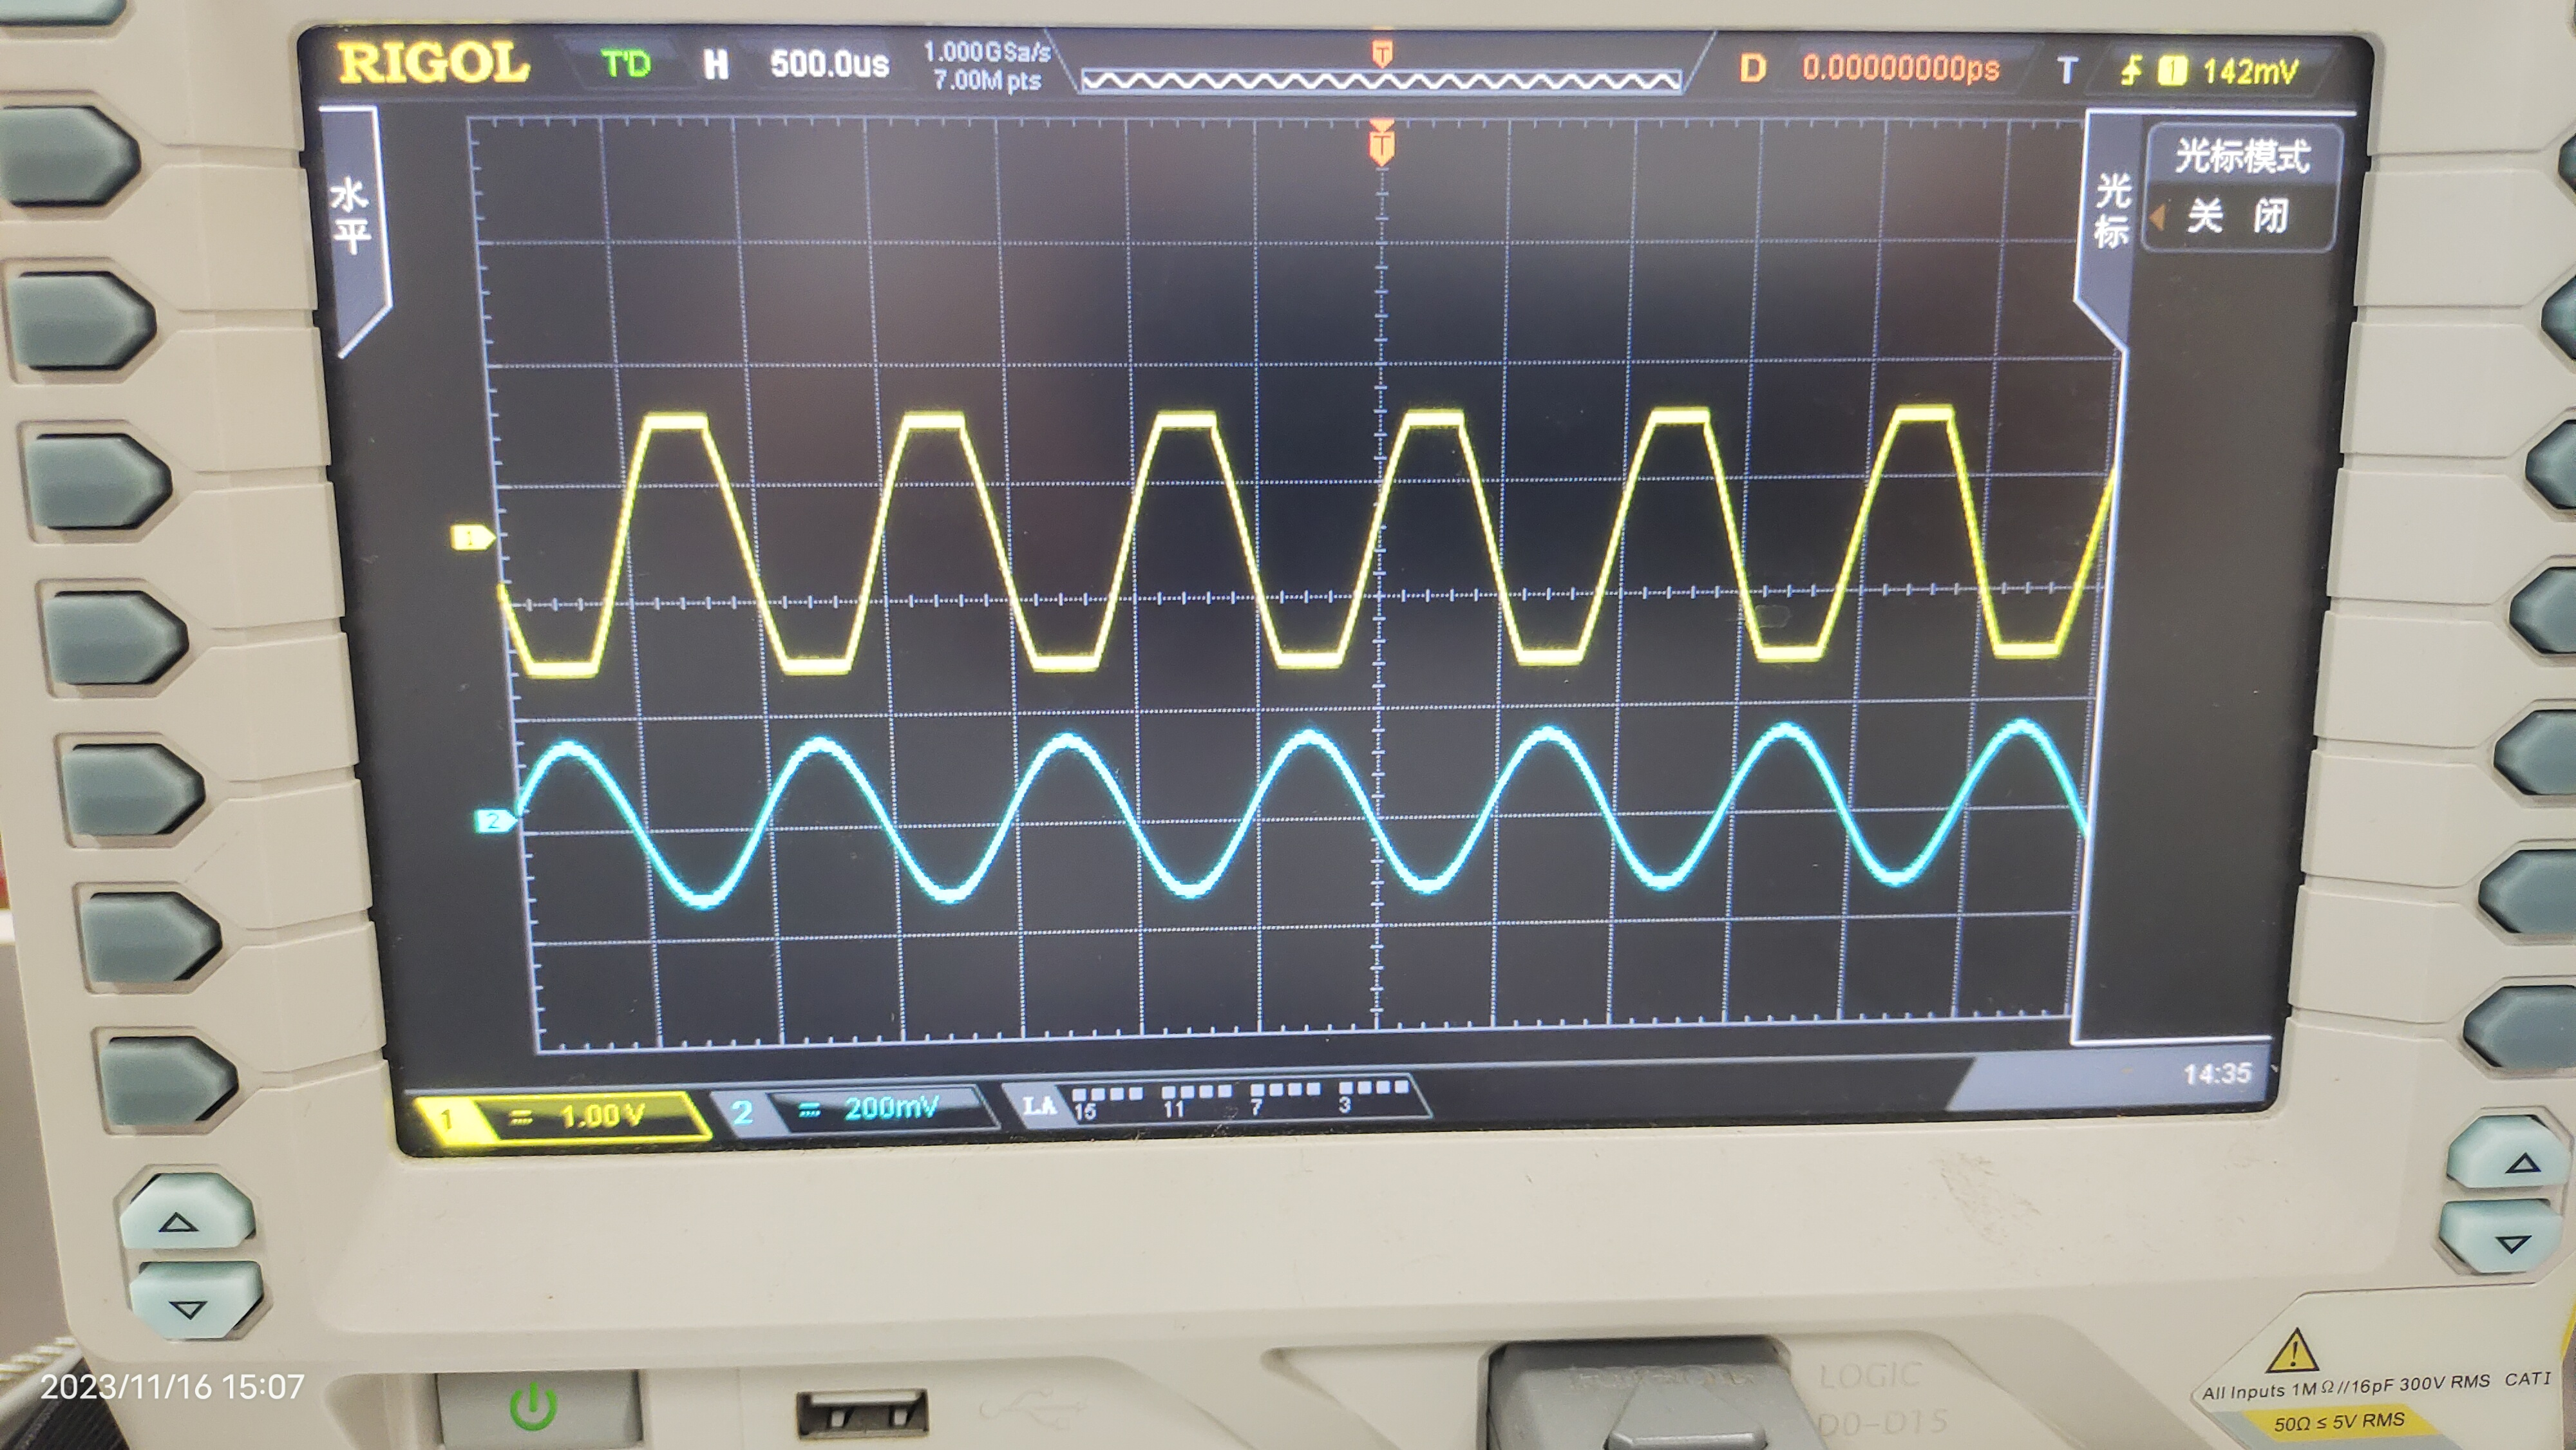
\includegraphics[width=\textwidth]{2.jpg}
					\caption*{图6-8 输入输出实验失真波形}
				\end{minipage}
			\end{figure}
		\end{enumerate}
		\item 同相比例放大器\par 
		按图6-2 连接电路。
		\begin{enumerate}
			\item 按给定直流输入信号,测量对应的输出电压,把结果记入表6-2 中。
			表6-2
			\begin{table}[h]
				\centering
				\begin{tabular}{|c|c|c|c|c|c|c|c|}
					\hline
					\multicolumn{2}{|c|}{$U_i(V)$} & 0.3 & 0.5 & 0.7 & 1.0 & 1.1 & 1.2 \\
					\hline
					理论计算值 & $U_O(V)$ & 3.01 & 5.01 & 7.01 & 10 & 11 & 11.1 \\
					\hline
					实际测量值 & $U_O(V)$ & 3.056 & 4.95 & 6.95 & 10.11 & 10.865 & 11.3 \\
					\hline
					实际放大倍数 & $A_{uf}$ & 10.187 & 9.9 & 9.93 & 10.11 & 9.88 & 9.417 \\
					\hline
				\end{tabular}
				\caption*{表6-2 同相比例放大器}
			\end{table}
			\item 在该比例放大器的输入端加入1KHz, 有效值为0.5V 的交流信号,用示波器观
			察输出波形,并与输入波形相比较。
			\newpage
			\begin{figure}[h]
				\raggedright
				\begin{minipage}{0.3\textwidth}
					\centering
					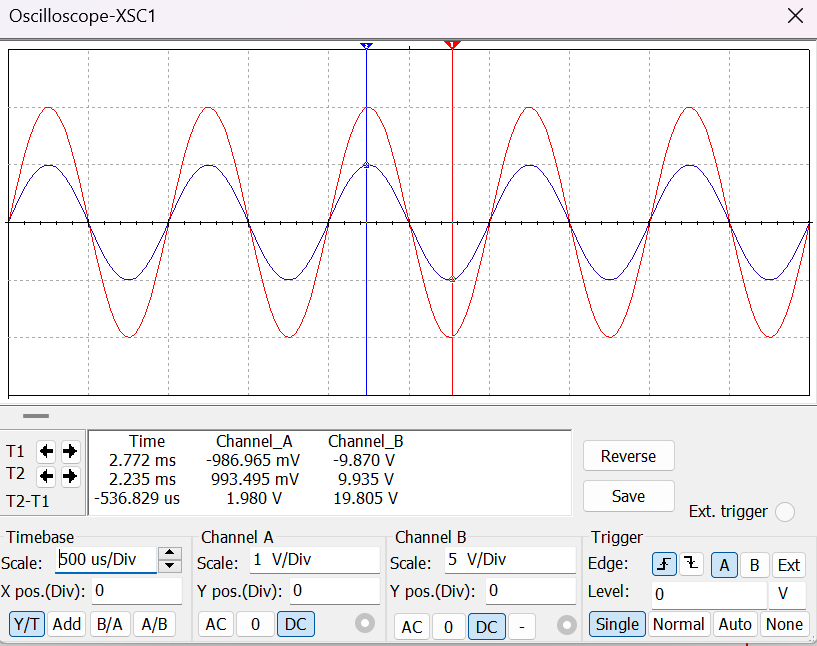
\includegraphics[width=\textwidth]{预习报告/6.png}
					\caption*{图6-9 输入输出仿真波形}
				\end{minipage}
				\qquad
				\begin{minipage}{0.3\textwidth}
					\centering
					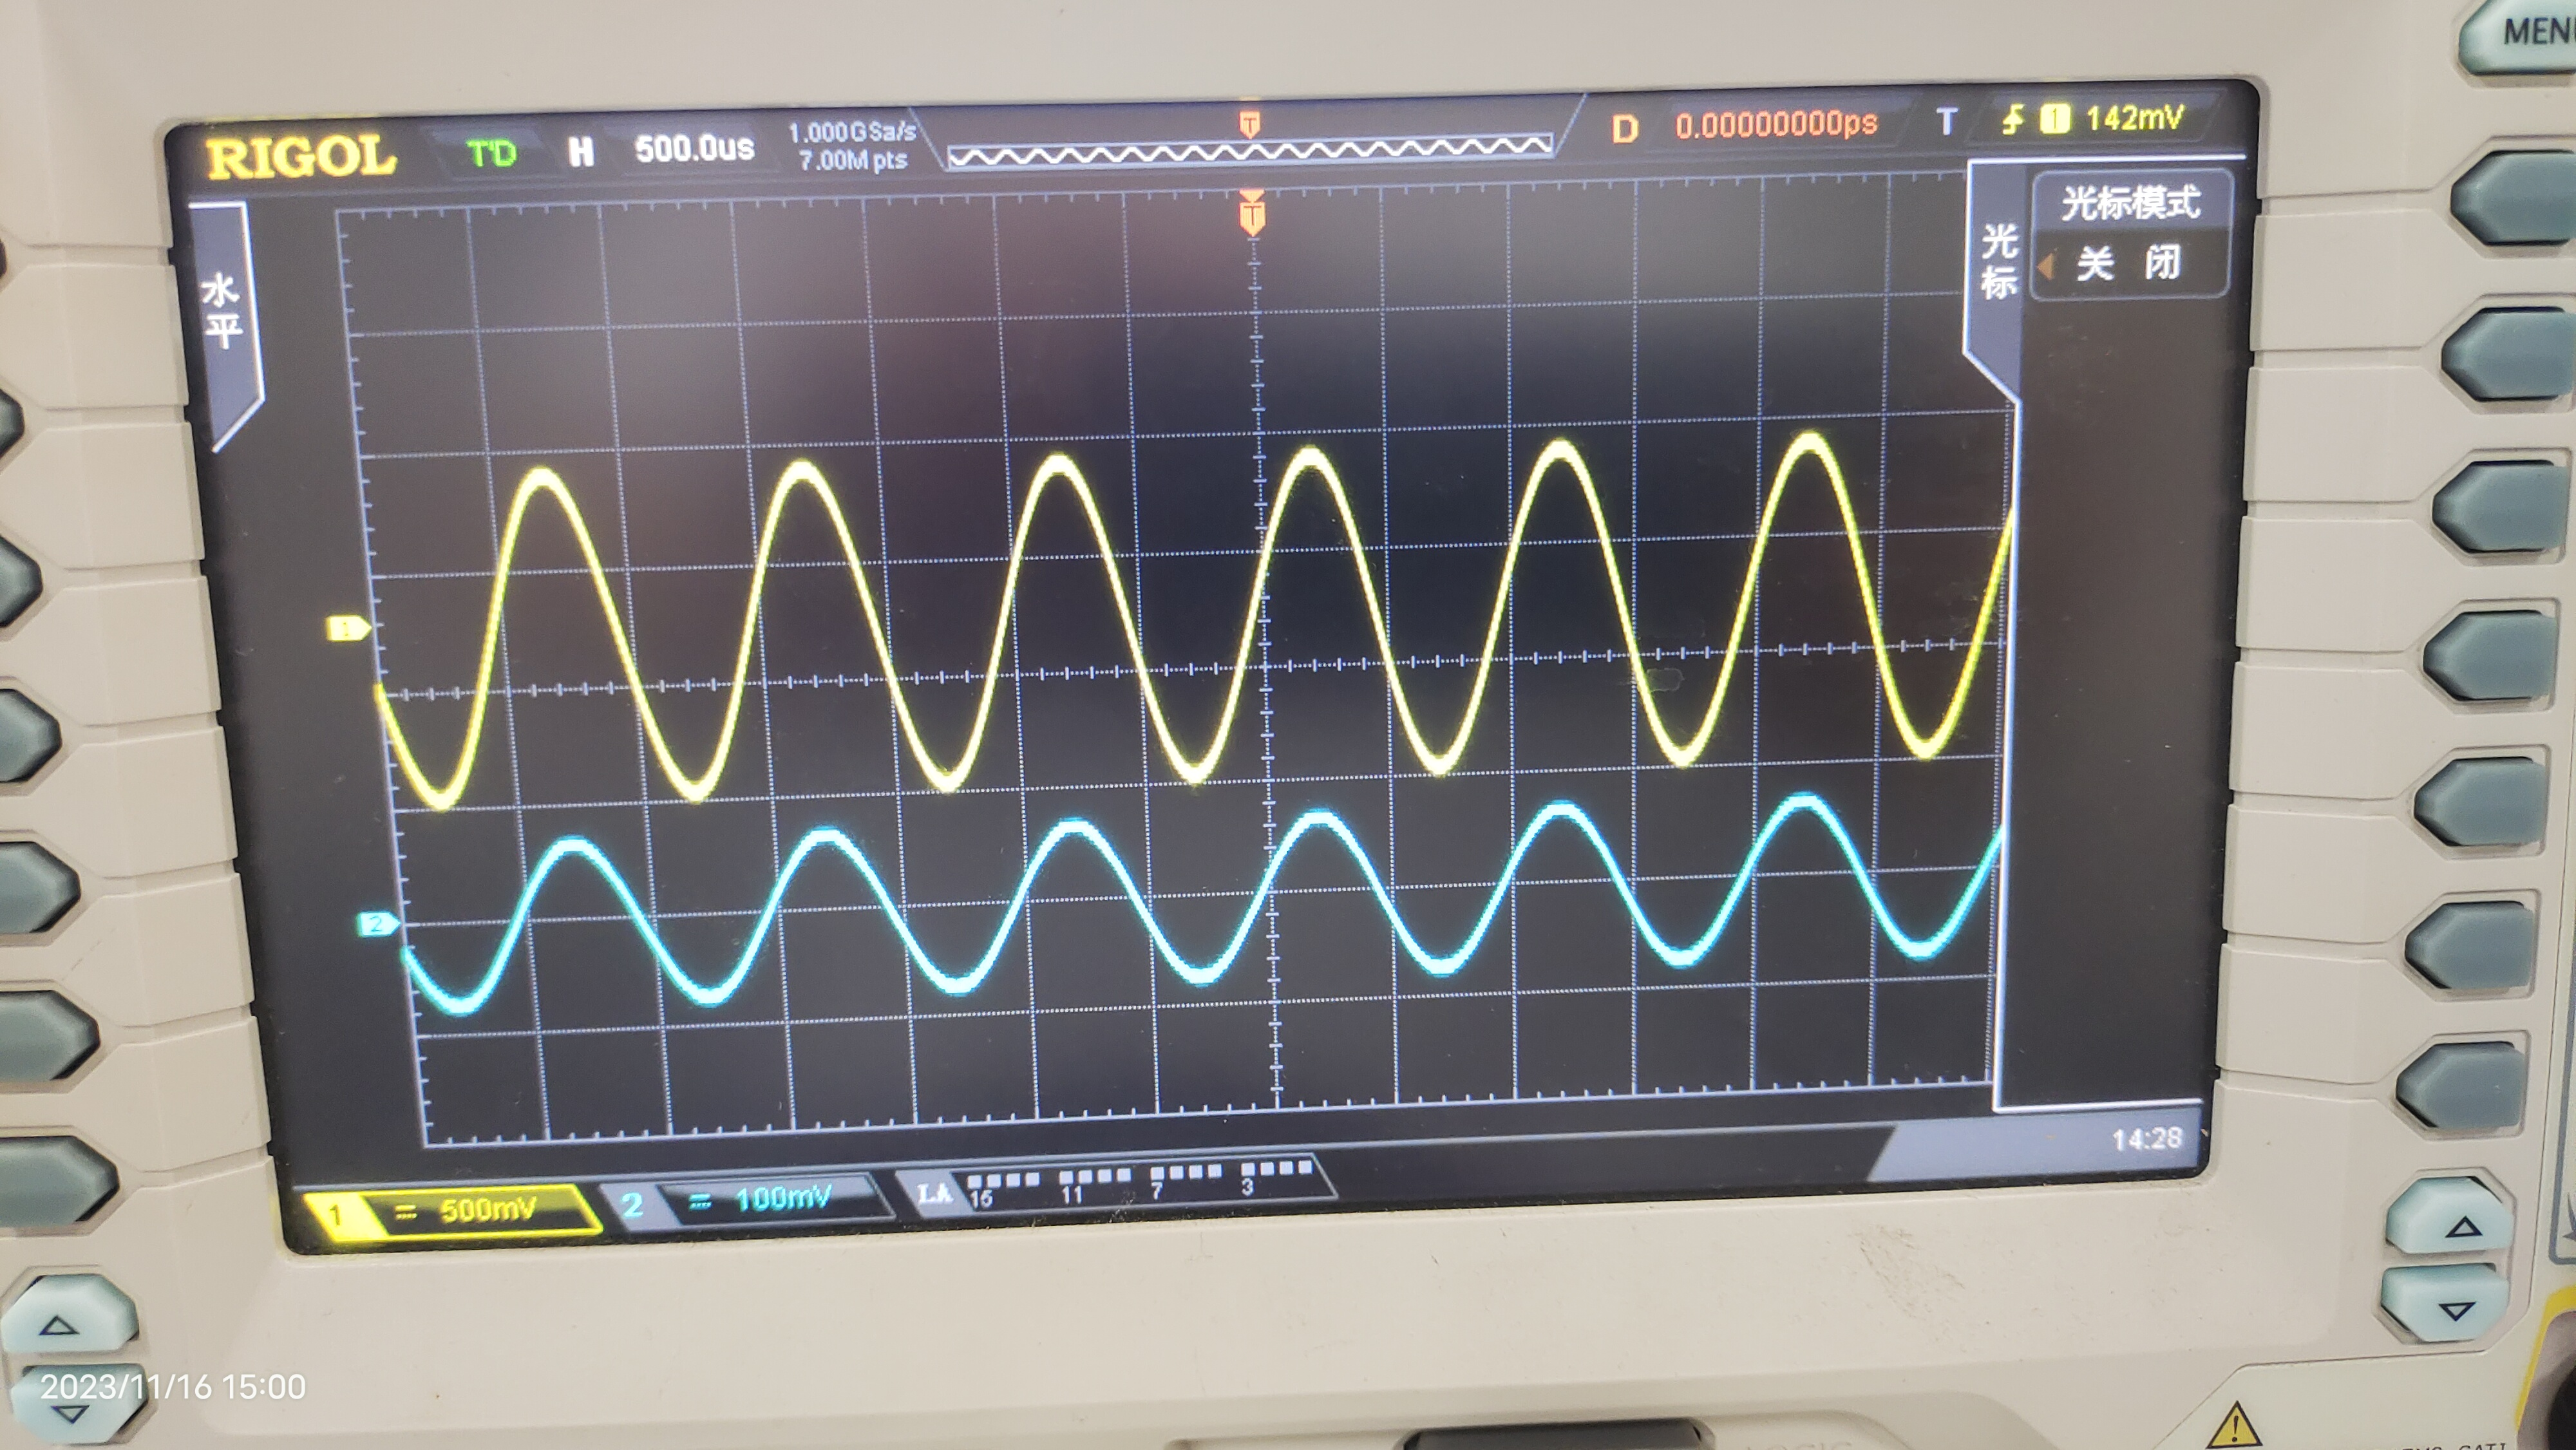
\includegraphics[width=\textwidth]{3.jpg}
					\caption*{图6-10 输入输出实验波形}
				\end{minipage}
				\qquad
				\begin{minipage}{0.3\textwidth}
					\centering
					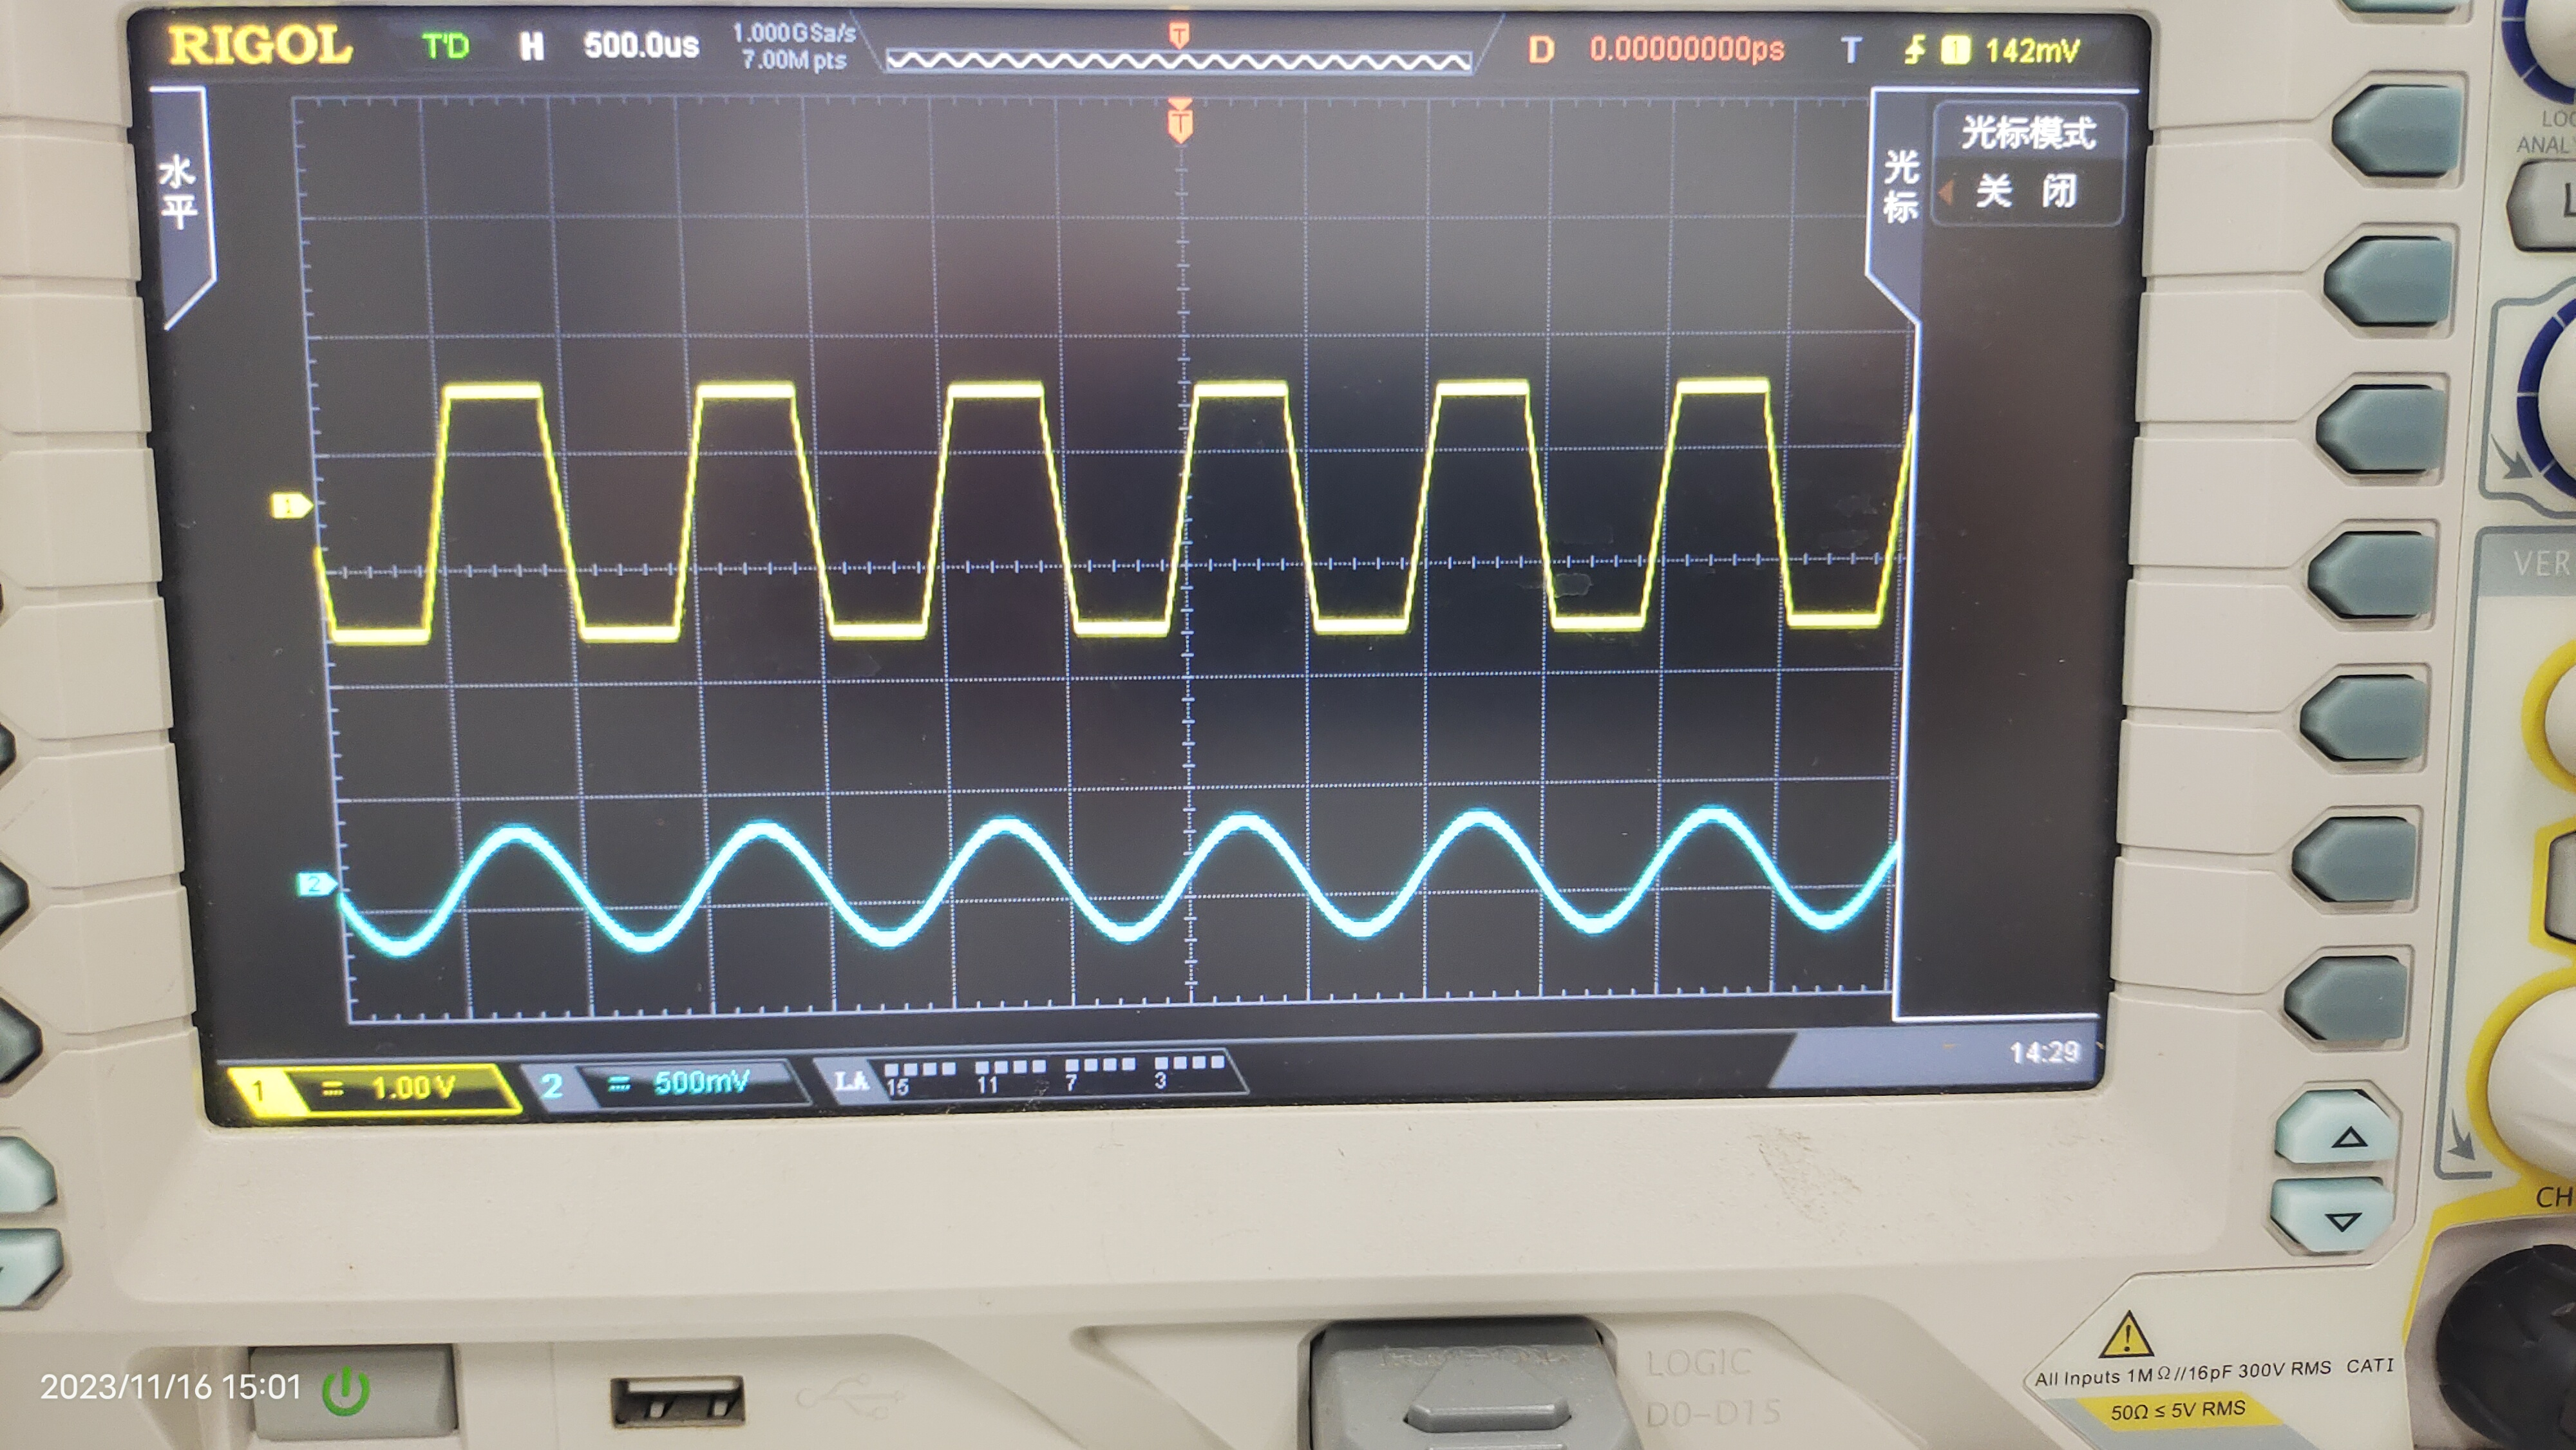
\includegraphics[width=\textwidth]{4.jpg}
					\caption*{图6-11 输入输出实验失真波形}
				\end{minipage}
			\end{figure}
		\end{enumerate}
		\item 减法器(差分比例运算)\par 
		\qquad 按图6-3 连接电路。按给定直流输入信号,测量对应的输出电压,把结果记入表6-3
		中。
		\begin{table}[h]
			\centering
			\begin{tabular}{|c|c|c|c|}
				\hline
				输入信号$U_{i1}(V)$ & 0.2 & 0.2 & -0.2 \\
				\hline
				输入信号$U_{i2}(V)$ & -0.3 & 0.3 & -0.3 \\
				\hline
				计算值$U_O(V)$ & -4.99 & 1.01 & -0.987 \\
				\hline
				实际测量值$U_O(V)$ & -5.02 & 0.981 & -9.88 \\
				\hline
			\end{tabular}
			\caption*{表6-3 减法器}
		\end{table}
		\item 反相加法器\par 
		\qquad 按图6-4 连接电路。同时将Ui1 与Ui2 对地短路,接通电源后,调节调零电位器
		Rp0(10K),使输出Uo=0。然后将短路线去掉,按给定直流输入信号,测量对应的输出电压,
		把结果记入表6-4 中。
		\begin{table}[h]
			\centering
			\begin{tabular}{|c|c|c|c|}
				\hline
				输入信号$U_{i1}(V)$ & 1.0 & 1.5 & -0.2 \\
				\hline
				输入信号$U_{i2}(V)$ & 0.4 & -0.4 & 1.2 \\
				\hline
				计算值$U_O(V)$ & -1.4 & -1.1 & -0.997 \\
				\hline
				实际测量值$U_O(V)$ & -1.397 & -1.09 & 1.02 \\
				\hline
			\end{tabular}
			\caption*{表6-4 反相加法器}
		\end{table}
		\item 加减法器\par 
		\qquad 按图6-5 连接电路。将3R10 与第一级运放的联接断开,按前述方法对两级分别进行
		调零。然后将短路线去掉,接好电路,按给定直流输入信号(Ui1 和Ui2 由同一信号源提
		供),测量对应的输出电压,把结果记入表6-5 中。
	\end{enumerate}
	\begin{table}[ht]
		\centering
		\begin{tabular}{|c|c|c|c|c|}
			\hline
			输入信号$U_{i1}(V)$ & $U_{i2}(V)$ & $U_{i3}(V)$ & 计算值$U_O(V)$ & 实际测量值$U_O(V)$ \\
			\hline
			0.4 & 0.8 & 0.4 & 11.1 & 11.101 \\
			\hline
		\end{tabular}
		\caption*{表5 加减法器}
	\end{table}
	\newpage
	\section*{五、实验总结}
	\begin{enumerate}
		\item 公式推导
		\begin{enumerate}
			\item 同向比例放大器的闭环电压增益公式推导\par 
			根据虚短和虚断,有:
			$$U_2=U_3=U_i$$
			由净输入电流为零:
			$$\frac{U_2-0}{R_1}=\frac{U_o-U_3}{R_{F}}$$
			由以上两式:
			$$U_o=(1+\frac{R_F}{R_1})U_i$$
			当放大倍数足够大时:
			$$U_o=\frac{R_F}{R_1}U_i$$
			得到放大倍数:
			$$A_{uf}=\frac{U_o}{U_i}=\frac{R_F}{R_1}$$
			\item 加减法器输出电压公式的推导\par 
			由于$U_{i1}$和$U_{i2}$相当于接入反向求和电路,所以
			$$U_{o1}=-R_{F1}(\frac{U_{i1}}{R_1}+\frac{U_{i2}}{R_2})$$
			由于第二级运算也是反向求和,所以
			$$U_{o}=-R_{F2}(\frac{U_{o1}}{10k}+\frac{U_{i3}}{R_2})$$
			又$R_{F1}=10k$,将上式代入得
			$$U_o=R_{F2}(\frac{U_{i1}}{R_1}+\frac{U_{i2}}{R_2}-\frac{U_{i3}}{R_3})$$
		\end{enumerate}
		\item 误差分析\par 
		\qquad 本次实验结果都较为合理,误差都在允许的范围内。
		\item 实验思考题
		\begin{enumerate}
			\item 运算放大器作比例放大时,R1 与RF 的阻值误差为±10%,试问如何分析和计算电
			压增益的误差?\par
			\qquad 根据电压增益公式可知,主要影响的是$R_F$和$R_1$的比值,因此,电压增益的误差区间为:
			$$(\frac{0.9R_F}{1.1R_1},\frac{1.1R_F}{0.9R_1})
			=\frac{R_F}{R_1}(0.818,1.375)$$
			\item 运算放大器作精密放大时,同相输入端对地的直流电阻要与反相输入端对地的直
			流电阻相等,如果不相等,会引起什么现象?\par 
			\qquad 可能会导致偏置电压漂移。因为放大器的输出在很大程度上取决于输入端的偏置电压,不匹配的输入电阻会导致不稳定的偏置,进而导致输出偏离预期值。同时也会导致共模抑制比下降,不匹配的输入电阻可能降低运算放大器的共模抑制比。这意味着放大器在抵抗共模信号(即同时应用于两个输入端的信号)时的效果不佳,可能导致输出中包含不必要的共模信号。还可能会导致偏置电流不平衡,输入电阻不匹配可能导致运算放大器两个输入端的偏置电流不平衡。这种不平衡可能影响放大器的性能,特别是在高增益应用中可能引起严重问题。
		\end{enumerate}
	\end{enumerate}
\end{document}